\documentclass[11pt,twoside]{report}

%\newif\ifmynotes
%\mynotesfalse
%\mynotestrue



\usepackage{ece586}

\usepackage{tikz}
\usetikzlibrary{positioning,angles,quotes}

%% TOGGLE  Notes
%\newif\ifgnotes
%\anstrue

%\ifmynotes
%	\definecolor{note_text}{rgb}{1,1,1}		
%	\newcommand{\gskip}{\vspace*{1cm}}
%	\newcommand\gnote[1]{\protect\leavevmode\begingroup\Huge\color{note_text}#1\endgroup\ignorespaces}
%	\newenvironment{gnotes}{\Huge\color{red}}{\ignorespacesafterend}
%\else
%	%\newcommand{\gnote}[1]{#1\ignorespaces} 	% make commands do nothing. 
%	\definecolor{note_text}{rgb}{0,0,.7}
%	\newcommand\gnote[1]{\protect\leavevmode\begingroup\color{note_text}#1\endgroup\ignorespaces}
%	\newenvironment{gnotes}{\color{red}}{\ignorespacesafterend}
%%	\newcommand{\gskip}{}
%\fi
%

\newcommand{\bbN}{{\mathbb{N}}}
\newcommand{\bbR}{{\mathbb{R}}}
\newcommand{\bbQ}{{\mathbb{Q}}}
\newcommand{\bbZ}{{\mathbb{Z}}}
\newcommand{\bbC}{{\mathbb{C}}}
\newcommand{\vecnot}{\underline}
\newcommand{\Id}{{\mathrm{I}}}

\newcommand{\Interior}[1]{\ensuremath{{#1}^{\circ}}}
\newcommand{\Closure}[1]{\ensuremath{\overline{#1}}}
\newcommand{\Complement}[1]{\ensuremath{{#1}^{c}}}

\newcommand{\Real}{\mathrm{Re}}
\newcommand{\Span}{\mathrm{span}}
\newcommand{\Rank}{\mathrm{rank}}
\newcommand{\Nullity}{\mathrm{nullity}}
\newcommand{\Trace}{\mathrm{tr}}
\newcommand{\Diag}{\mathrm{diag}}

\begin{document}

\lectureheader{4}{Markov Chains}



\section*{Overview} 

\begin{itemize}
%\item In this lecture, we consider noisy linear observation model
% \[
% \by = A \bx^\star + \be
% \]
% where:
%\begin{itemize}
%\item $\bx^\star$ is an unknown $n$-dimensional vector belonging to a set $\cX \subseteq \reals^n$. 
%\item $A$ is an $m \times n$ measurement matrix
%\item $\be$ is and $m$-dimensional vector of measurement errors
%\end{itemize}


\item Some background for this lecture can be found in  \cite[Chapter~4]{durrett:2012} and \cite[Chapter~5]{durrett:2019}.
% and \cite[Parts~I--II]{bloch:2011}


\end{itemize}

%\section{Introduction} 
%
%%\section{Logic Systems} 
%
%\begin{itemize}
%\item Linear algebra is the foundation of engineering mathematics 
%  \begin{itemize}
%  \item This chapter will review and extend your knowledge of linear algebra
%  \item Abstraction allows the application of similar ideas to many different areas
%  \item Your prior experience with real vector spaces makes this possible 
%  \end{itemize}
%\item Abstraction 
%  \begin{itemize}
%  \item Metric spaces provide abstract notions of distance and closeness
%  \item Fields provide abstract notions for arithmetic of scalars ($+,-,\times,/$)
%  \item Vector spaces abstract the additive properties of real vectors
%  \end{itemize}
%  \end{itemize}
%  
%  
\section{Markov Chains}

\begin{itemize}

\item %\textbf{Definition} 
A \textbf{finite-state Markov chain}  (FSMC) with $n$ states is a sequence of random variables $X_{1},X_{2},X_{3},\ldots$  taking values in the set $[n]\coloneqq  \{ 1,2,\ldots,n \} $ where
\[
\pr{ X_{t+1}=j \mid X_{t}=i,X_{t-1} = i_{t-1} , \dots, X_{1} = i_1 } =\pr{ X_{t+1}=j\,\middle|\,X_{t}=i} 
\]
for possible values of  $i_1, \dots, i_{t-1},i,j \in [n]$

%\item A discrete-time stochastic process $\{X_1, X_2, \dots \}$ is said to be a {\em Markov chain} or {\em Markov process} if for all $n=1,2,\dots,$ 
%  \ifans  \clearpage \else  
%\[
%\pr{X_{n+1} = x_{n+1} | X_{n} = x_n, X_{n-1}  = x_{n-1}, \cdots, X_1 = x_1}  = \pr{X_{n+1} = x_{n+1} | X_n = x_n}
%\]
%for all $x^{n+1} \in \cX^{n+1}$. 
%\fi
%Thus, the probability of state $X_{n+1}$ is given by
%\[
%\pr{X_{n+1} = x}= \sum_{x' \in \cX} \pr{X_n = x'}\pr{X_{n+1} = x | X_{n} = x'}
%\]


\item A Markov chain is \textbf{time-invariant} if the conditional probability $\pr{ X_{t+1}=j\,\middle|\,X_{t}=i} $ does not depend on $t$, i.e.  
\[
\pr{X_{t+1} =j \mid  X_t = i} = \pr{X_2 = i \mid  X_1 = j} \qquad \text{for all $i,j \in [n]$}
\]


  \ifans  \vspace*{2in}\else  
\item For time-invariant Markov chain on $n$ is states, the \textbf{transition probability  matrix } is the $n \times n$ matrix $P$ defined by
\[
P_{i,j} = \pr{X_{t+1} = j \mid  X_t= i}, \qquad i,j \in [n]
\]
\item  Note that  each \emph{row} of $P$ is a probability distribution, i.e., % Hence, $P$ is a row-stochastic matrix, i.e.,  a matrix whose entries are non-negative and whose rows sum to one:
 \[
 P_{i,j}\geq0 \quad \text{and} \quad  \sum_{j=1}^{n}P_{i,j}=1, \quad \text{for all $i$}
\]
A matrix with non-negative entries and rows that sum to one is called \textbf{stochastic}. 


%The vector of probabilities at time $n$ is denote by
%\[\mu_{n} = (\pr{X_{n} = 1}, \pr{X_{n} = 2}, \dots, \pr{X_{n} = M} )\]
%and is updated according to 
%\[
%\mu_{n+1}  = \mu_{n}  P
%\]
%\fi

\item {\bf Example:} Consider the  time-invariant Markov chain on $n=3$ states with transition probability matrix
\[
%\pr{X_{n+1} = j | X_{n} = i} = [P]_{i,j} \qquad \text{with} \qquad
 P = \begin{bmatrix}
1-\alpha & \alpha & 0\\
\beta & 1- \alpha - \beta & \alpha\\
0 & \beta & 1-\beta
\end{bmatrix}
\]

%\vspace{1 in}

  \ifans  \vspace*{3in}\else  

\begin{center}
  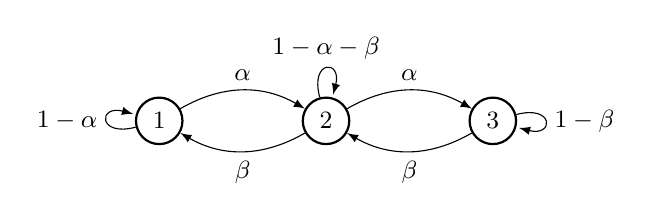
\begin{tikzpicture}[auto,node distance=8mm,>=latex,font=\small]

    \tikzstyle{round}=[thick,draw=black,circle]

    \node[round] (n1) {$1$};
    \node[round, right = 1.5cm of n1] (n2) {$2$};
    \node[round, right=1.5cm of n2] (n3) {$3$};
    
    \path[->]  
     (n1)  edge[bend left,"$\alpha$"] (n2)
     (n2)  edge[bend left,"$\alpha$"] (n3)
     (n3)  edge[loop right,"$1-\beta$"] (n3)
     (n2)  edge[loop above,"$1-\alpha - \beta$"] (n2)
    (n3) edge[bend left, "$\beta$"] (n2)
    (n2) edge[bend left, "$\beta$"] (n1)
    (n1) edge[loop left, "$1-\alpha$"] (n1);
     

 %   \draw[->] (n1) [out = -40, in = -140] to (n2) node [midway, below]{$\beta$};
%    \draw[->] (s0) -- (s2);
%    \draw[->] (s0) [out=40,in=100,loop] to coordinate[pos=0.1](aa) (s0);
%    \path pic[draw, angle radius=6mm,"\vphantom{g}a",angle eccentricity=1.2] {angle = s2--s0--aa};
\end{tikzpicture}
\end{center}
\fi
%
%\begin{itemize}
%%
%%\item The probability of state $X_{n+1}$ is given by
%%$$\pr{X_{n+1} = j}= \sum_{i =1}^3 \pr{X_n = i}\pr{X_{n+1} = j | X_{n} = i}$$ or more conveniently $$\mu_{n+1} = \mu_n P$$
%%where
%%\[\mu_{n} = (\pr{X_{n} = 1}, \pr{X_{n} = 2}, \pr{X_{n} = 3} )\]
%
%
%
%\item The stationary distribution $\mu$ is given by the vector that satisfies
%\[\pr{X_{n+1} = j}= \sum_{i =1}^3 \pr{X_n = i}\pr{X_{n+1} = j | X_{n} = i}\]
%or equivalently
%\[
%\mu = \mu P 
%\]
%%
%%a distribution $p(x)$ is stationary if $p(x_n)$ does not depend on $n$, and hence
%%$$p(x_{n+1}) = \sum_{x_n} p(x_n) P(x_{n_1}|x_{n})$$
%%or $$ \mu = \mu P$$
%
%In this cases, the stationary distribution is
%$$ \mu = \left( \frac{1}{1 + r + r^2}, \frac{1}{r^{-1} + 1 + r}, \frac{1}{r^{-2} + r + 1}\right)$$
%where $r = \alpha / \beta$. Note that if $\alpha = \beta$, then this is the uniform distribution. 
%\end{itemize}


\item The probability mass function (pmf) for  $X_t$  is denoted by the $n \times 1$ row vector 
\[
\vecnot{\pi}^{(t)} = (\pi_{1}^{(t)},\ldots,\pi_{n}^{(t)}) \quad \text{where} \quad \pi_{i}^{(t)}\coloneqq \pr{ X_{t}=i} 
\]

\item \textbf{Lemma:}  The distribution of a time-invariant Markov chain  $X_1, X_2, X_3, \dots, $ is completely specified by the marginal distribution  of the first time step $\vecnot{\pi}^{(1)}$ and  the transition probability matrix $P$.  
%\begin{enumerate}[(1)]
%\item the transition probability matrix $P$
%\item the distribution $\vecnot{\pi}^{(1)}$ of  $X_1$.  
%\end{enumerate}
Moreover, 
\begin{itemize}
\item the pmf of state $t$ satisfies
\[
\pi^{(t+1)}  = \pi^{(1)} P^t , \qquad \text{where} \quad P^t = \underbrace{P P \cdots P}_\text{$t$ times}% , \quad \text{for all $t \in \bbN$}
\]
\item the multistep transition probability is 
\[
\pr{ X_{t+1} = j \mid X_1 = i} =[ P^t]_{i,j}
\]
where $[P^t]_{i,j}$ denotes  entry $(i,j)$ of the $n \times  n$ matrix $P^t$.
\end{itemize}
\item \textbf{Proof:} 
\begin{itemize}
\item The  distribution of $X_{t+1}$ can be computed as 
\begin{align*}
%\pi_{j}^{(t+1)} & =
 \pr{ X_{t+1} =j } 
& =\sum_{i=1}^{n}\pr{X_t = i,  X_{t+1}=j} \\
 & =\sum_{i=1}^{n} \pr{ X_{t}=i} \underbrace{ \pr{ X_{t+1}=j \mid X_{t}=i}}_{P_{i.j}}  %\\
% & =\sum_{i=1}^{n} P_{i,j} \pi_{i}^{(t)}
\end{align*}
\item Using, matrix vector notation, this relationship can be written succinctly as 
\[
\pi^{(t+1)}   = \pi^{(t)}  P 
\]
\item By induction it follows that
\begin{align*}
\pi^{(t+1)}  &  = \pi^{(t)}  P \\
&  = \pi^{(t-1)}  P^2\\
&  = \pi^{(t-2)}  P^3\\
&\quad  \vdots\\
& = \pi^{(1)} P^t  
%\pi_{j}^{(t+1)} & =\sum_{i=1}^{n}\pr{ X_{t+1}=j,X_{t}=i} \\
 %& =\sum_{i=1}^{n} \pr{ X_{t+1}=j \mid X_{t}=i} \pr{ X_{t}=i}\\
 %& =\sum_{i=1}^{n} \pr{ X_{t+1}=j \mid X_{t}=i} \pi_{i}^{(t)}\\%\pr{ X_{t}=i}\\
 %& =\sum_{i=1}^{n}P_{i,j}\pi_{i}^{(t)}=\left[\vecnot{\pi}^{(1)}P^{t}\right]_{j}
\end{align*}
\end{itemize}


\end{itemize}

%\subsection{Simulating Markov chaines} 

\subsection{Hitting times} 

\begin{itemize}

\item \textbf{Definitions:} For a time-invariant Markov chain with transition probability matrix $P$, 
\begin{itemize}
\item state $j$ is \textbf{reachable} from state $i$ if  %there exists 
\[
\exists m \in \bbN \quad \text{such that} \quad [P^m]_{i,j}  >0
\]
i.e.,  a chain starting at state $i$ has positive probability of reaching state $j$ at some point in the future

\item state $j$ is \textbf{absorbing} if $P_{j,j}  =1$, i.e., once the chain reaches state $j$ it never leaves.
\end{itemize}

\item  For a Markov chain starting from state $X_1 = i$, the first \textbf{hitting time} of state $j$ is the random variable
\[
T_{i,j} \coloneqq \inf\{ m \in \bbZ_{\ge 0} \mid  X_{m+1}=j \} 
\]
Note that $T_{i,i} = 0$ and $T_{i,j} = \infty$ if state $j$ is not reachable from state $i$. 
%By convention, $\pr{ T_{i,j}=0 } =\delta_{i,j}$ where $\delta_{i,j}$ is Kronecker delta function and,  if state $j$ is not reachable from state $i$, then $T_{i,j} = \infty$. 
%\item 
\item The probability mass function (pmf) of of the first hitting time satisfies
%\[
%\pr{ T_{i,j}=m} =
% \pr{ X_{m+1}=j,X_{m}\neq j,X_{m-1}\neq j,\ldots,X_{2}\neq j \mid X_{1}=i } , 
%\]
\[
\pr{ T_{i,j}=m} =
 \pr{ ( X_{m+1}=j ) \wedge ( \forall s \in \{ 1, \dots, m\}  \,, \,   X_{s}\ne j )   \mid X_{1}=i } , 
\]
In particular, $\pr{T_{i,j} = 0} = \delta_{i,j}$ where $\delta_{i,j}$ is the Kronecker delta function. 
%for all $m \in \bbZ_{\ge 0}$. 
%for $m = 0,1, 2,\dots$. 
%By convention, $\pr{ T_{i,j}=0 } =\delta_{i,j}$ where $\delta_{i,j}$ is Kronecker delta function and,  if state $j$ is not reachable from state $i$, then $T_{i,j} = \infty$. 
%Let the cumulative distribution function (cdf) be denoted by
%\[
%\phi_{i,j}^{(m)} = \pr{ T_{i,j} \le m} 
%\]


%\item For a Markov chain starting from state $i$, the first \textbf{hitting time} of state $j$ is a random variable $T_{i,j}$ with distribution 
%\[
%\pr{ T_{i,j}=m} = \pr{ X_{m+1}=j,X_{m}\neq j,X_{m-1}\neq j,\ldots,X_{2}\neq j \mid X_{1}=i } 
%\]
%\item By convention, $\pr{ T_{i,j}=0 } =\delta_{i,j}$ where $\delta_{i,j}$ is Kronecker delta function and,  if state $j$ is not reachable from state $i$, then $T_{i,j} = \infty$.
%Alternatively, we have
%\vspace{-2mm}
%\[
%\pr{ T_{i,j} \leq m} =\pr{ \exists t \in \{1,2,\ldots,m+1\}, X_{t}=j  \mid X_{1}=i } 
%\]
%
%
%\item A state $j$ is an \textbf{absorbing state} if $P_{j,j}  =1$. One the chain reaches an absorbing state is never leaves.


%\[
%\pr{ T_{i,j} \le m}  =\pr{ X_{m+1}  = j \mid X_1 = i}  = [ P^m]_{i,j} 
%\]

%\item \textbf{Proof:} 
%\[
%\phi_{i,j}^{(m+1)} = \pr{ T_{i,j}\leq m+1} =\begin{dcases}
%1, & i=j\\
%\sum_{k=1}^{n}P_{i,k}\pr{ T_{k,j}\leq m} , & i \ne j
%\end{dcases}
%\]

\item \textbf{Lemma:}
 If $j$ is an absorbing state then the cdf of the first hitting time is given by
\[
\pr{ T_{i,j} \le m}   = [ P^m]_{i,j} 
\]
and thus the pmf is given by
\[
\pr{ T_{i,j}=m} =\left[P^{m}-P^{m-1}\right]_{i,j}.
\]

\item \textbf{Proof} 
\begin{itemize}
\item  The fact that $j$ is absorbing means that $X_{t+1} = j$ for all $t \ge T_{i,j}$ and thus
\[
T_{i,j} \le m \quad \implies  \quad X_{m+1}  = j 
\]
\item On the other hand, from definition of first hitting time, 
\[
T_{i,j} \le m \quad \impliedby \quad X_{m+1}  = j 
\]
\item Therefore, $T_{i,j} \le m$ if and only if $X_{m+1}  = j $ and so the cdf satisfies
\[
\pr{ T_{i,j} \le m}  =\pr{ X_{m+1}  = j \mid X_1 = i}  = [ P^m]_{i,j} 
\]
where the second  equality is the formula for the multistep transition probability
\end{itemize}


\item \textbf{Lemma:} For a time-invariant Markov chain with transition probability matrix $P$, the distribution of the first hitting time satisfies the recursion 
\begin{align*}
\pr{T_{i,j} = 0}  & = \delta_{i,j}\\
\pr{T_{i,j} = m} & =(1-\delta_{i,j})\sum_{k=1}^{n}P_{i,k}\pr{T_{k,j} = m-1} , \quad \text{for $m =  1,2,3,\dots$} 
\end{align*}
%for all $ m  = 0,1,2,\dots $,   
where $\delta_{i,j}$ is the Kronecker delta function. 



\item \textbf{Corollary:} The cdf of the first hitting time $\phi_{i,j}^{(m)} \coloneqq \pr{ T_{i,j} \le m} $  satisfies the recursion 
\begin{align*}
\phi_{i,j}^{(0)} & = \delta_{i,j}\\
\phi_{i,j}^{(m)} & =\delta_{i,j}+(1-\delta_{i,j})\sum_{k=1}^{n}P_{i,k}\phi_{k,j}^{(m-1)},  \quad \text{for $m = 1,2,3,\dots$} %\qquad  \text{for $m \in \bbZ_{\ge 0} $} 
\end{align*}
%for all $ m  = 0,1,2,\dots $,   where $\delta_{i,j}$ is the Kronecker delta function. 

\item \textbf{Proof:} 

\begin{itemize}
%\item Case $m=0$ follows from the fact that $T_{i,j} = 0$ if and only if  $i =j$.
%
%
%\item Case $m =1 $ follows form
%\begin{align*}
%\phi_{i,j}^{(1)} & = \pr{ T_{i,j} \le 1}  \\
%& = \pr{ T_{i,j} = 0} + \pr{ T_{i,j} =  1}\\
%& =\delta_{i,j}  +(1- \delta_{i,j})  \pr{ X_2 = j \mid X_1 = i}\\
%& =\delta_{i,j}  +(1- \delta_{i,j}) P_{i,j} \\
%& =\delta_{i,j}  +(1- \delta_{i,j})  \sum_{k=1}^n P_{i,k}  \delta_{k,j} \\
%& =\delta_{i,j}  +(1- \delta_{i,j})  \sum_{k=1}^n P_{i,k}  \phi_{k,j}^{(0)} 
%\end{align*}
%
%\item If $i = j$ then $\phi_{i,j}^{(m)} = 1$ for all $m$. 
%
%\item For $i \ne j$, we can consider all possible values of $X_2$ to write: 
%\begin{align*}
% \pr{ T_{i,j} \le m+1}   & =  \sum_{k=1}^n  \pr{ T_{i,j} \le m+1 , X_2 = k }\\
% & =  \sum_{k=1}^n \pr{X_2 = k \mid X_1 = i}  \pr{ T_{i,j} \le m+1 \mid X_2 = k }\\
%  & =  \sum_{k=1}^n  P_{i,j}   \pr{ T_{k,j} \le m  }\\
%%& =\delta_{i,j}  +(1- \delta_{i,j})  \pr{ X_2 = j \mid X_1 = i}\\
%%& =\delta_{i,j}  +(1- \delta_{i,j}) P_{i,j} \\
%%& =\delta_{i,j}  +(1- \delta_{i,j})  \sum_{k=1}^n P_{i,k}  \delta_{k,j} \\
%%& =\delta_{i,j}  +(1- \delta_{i,j})  \sum_{k=1}^n P_{i,k}  \phi_{k,j}^{(m)} 
%\end{align*}
%Here, the key step is the last line which holds because 
%%

\item The case $m = 0$ holds since $T_{i,j} = 0$ if and  only if $i = j$. 
\item For $m  \in \bbN$, we can condition on the all possible values of $X_2$ to write
\begin{align*}
%&
 \pr{ T_{i,j}=m}
& =  \pr{ ( X_{m+1}=j ) \wedge ( \forall s \in \{ 1, \dots, m\}  \,, \,   X_{s}\ne j )   \mid X_{1}=i } \\
& =  \sum_{k=1}^n  \pr{ ( X_{m+1}=j ) \wedge ( \forall s \in \{ 1, \dots, m\}, \,   X_{s}\ne j ) \wedge (X_2 = k)   \mid X_{1}=i } \\
&=\sum_{k=1}^n  P_{i,k}  \pr{ ( X_{m+1}=j ) \wedge ( \forall s \in \{ 1, \dots, m\} , \,   X_{s}\ne j )   \mid X_{2}=k , X_1  = i } \\
& =  (1 - \delta_{i,j}) \sum_{k=1}^n  P_{i,k}  \pr{ ( X_{m+1}=j ) \wedge ( \forall s \in \{ 2, \dots, m\} , \,   X_{s}\ne j )   \mid X_{2}=k  } \\
&\overset{\mathrm{(a)}}{ =}    (1 - \delta_{i,j}) \sum_{k=1}^n  P_{i,k}  \pr{ ( X_{m}=j ) \wedge ( \forall s \in \{ 1, \dots, m-1\} , \,   X_{s}\ne j )   \mid X_{1}=k  } \\
& =  (1 - \delta_{i,j}) \sum_{k=1}^n  P_{i,k}  \pr{ T_{k,j} = m -1 } , 
\end{align*}
Step (a) follows from the time invariance of the Markov chain. 
%
%For $m \in \bbN$ and $i \ne j$ we have
%\begin{align*}
%& \pr{ T_{i,j}=m}\\
%& =  \pr{ ( X_{m+1}=j ) \wedge ( \forall s \in \{ 2, \dots, m\}  \,, \,   X_{s}\ne j )   \mid X_{1}=i } \\
%& =  \sum_{k=1}^n  \pr{ ( X_{m+1}=j ) \wedge ( \forall s \in \{ 2, \dots, m\}  \,, \,   X_{s}\ne j ) \wedge (X_2 = k)   \mid X_{1}=i } \\
%& =  \sum_{k=1}^n  P_{i,k}  \pr{ ( X_{m+2}=j ) \wedge ( \forall s \in \{ 2, \dots, m\}  \,, \,   X_{s}\ne j )   \mid X_{2}=k } \\
%& =  (1 - \delta_{i,j}) \sum_{k=1}^n  P_{i,k}  \pr{ ( X_{m+2}=j ) \wedge ( \forall s \in \{ 2, \dots, m\}  \,, \,   X_{s}\ne j )   \mid X_{2}=k  } \\
%& =  (1 - \delta_{i,j}) \sum_{k=1}^n  P_{i,k}  \pr{ ( X_{m+1}=j ) \wedge ( \forall s \in \{ 1, \dots, m-1\}  \,, \,   X_{s}\ne j )   \mid X_{1}=k  } \\
%& =  (1 - \delta_{i,j}) \sum_{k=1}^n  P_{i,k}  \pr{ T_{k,j} = m -1 } , 
%\end{align*}
%
%%
%or
%\begin{align*}
%& \pr{ T_{i,j}=m+1}\\
%& =  \pr{ ( X_{m+2}=j ) \wedge ( \forall s \in \{ 1, \dots, m+1\}  \,, \,   X_{s}\ne j )   \mid X_{1}=i } \\
%& =  \sum_{k=1}^n  \pr{ ( X_{m+2}=j ) \wedge ( \forall s \in \{ 1, \dots, m+1\}  \,, \,   X_{s}\ne j ) \wedge (X_2 = k)   \mid X_{1}=i } \\
%& =  \sum_{k=1}^n  P_{i,k}  \pr{ ( X_{m+2}=j ) \wedge ( \forall s \in \{ 1, \dots, m+1\}  \,, \,   X_{s}\ne j )   \mid X_{2}=k , X_1  = i } \\
%& =  (1 - \delta_{i,j}) \sum_{k=1}^n  P_{i,k}  \pr{ ( X_{m+2}=j ) \wedge ( \forall s \in \{ 2, \dots, m+1\}  \,, \,   X_{s}\ne j )   \mid X_{2}=k  } \\
%& =  (1 - \delta_{i,j}) \sum_{k=1}^n  P_{i,k}  \pr{ ( X_{m+1}=j ) \wedge ( \forall s \in \{ 1, \dots, m\}  \,, \,   X_{s}\ne j )   \mid X_{1}=k  } \\
%& =  (1 - \delta_{i,j}) \sum_{k=1}^n  P_{i,k}  \pr{ T_{k,j} = m  } , 
%\end{align*}
%
%
%\item Assume that the recursion is valid up to time $m$. Observe that for all $i \ne j$, 
%\begin{align*}
%& \pr{ T_{i,j} =  m+1} \\
% & = (1- \delta_{i,j})  \pr{ X_{m+2}=j, X_{m+1} \ne j , X_{m}\neq j,\ldots,X_{2}\ne j \mid X_{1}=i } \\
%&  =(1- \delta_{i,j})  \sum_{k =1 }^n  (1- \delta_{i,k})  \pr{ X_{m+2}=j, X_{m+1} \ne j , X_{m}\neq j,\ldots,X_{3} \ne j, X_{2} = k \mid X_{1}=i } \\
%&  =(1- \delta_{i,j})   \sum_{k \ne j } ( 1- \delta_{i,k})   P_{i,k}  \pr{ X_{m+2}=j, X_{m+1} \ne j , X_{m}\neq j,\ldots,X_{3} \ne j \mid X_{2} = k} \\
%&  =(1- \delta_{i,j})   \sum_{k \ne j } ( 1- \delta_{i,k})   P_{i,k}  \pr{ X_{m+2}=j, X_{m} \ne j , X_{m-1}\neq j,\ldots,X_{2} \ne j \mid X_{1} = k} \\
%&  =(1- \delta_{i,j})   \sum_{k \ne j } P_{i,k}  \pr{ T_{k,j} = m} 
%%&  = \sum_{k \ne j }   P_{i,k}  \pr{ X_{m+1}=j, X_{m} \ne j , X_{m-1}\neq j,\ldots,X_{2} \ne j \mid X_{1} = k}  \\
%%&  = \sum_{k \ne j }   P_{i,k}  \pr{ T_{k,j} =  m} \\
%%&  = -  P_{j,j}  \pr{ T_{i,j} =  m} +    \sum_{k =1 }^n   P_{i,k}  \pr{ T_{k,j} =  m}  
%\end{align*}
%Hence,
%\begin{align*}
%\phi_{i,j}^{(m+1)} & =\pr{ T_{i,j} =  0} + \pr{ T_{i,j} =  1} +  \sum_{ s= 1}^{m} \pr{ T_{i,j} =  s+1}\\
%&  = \delta_{i,j} +  (1 - \delta_{i,j})   P_{i,j}   +  \sum_{ s= 1}^{m}  \sum_{k= 1}^n (1 - \delta_{j,k})    P_{i,k}  \pr{ T_{k,j} =  s} \\
%&  = \delta_{i,j} +  \sum_{k= 1}^n   (1 - \delta_{j,k})     P_{i,k}   \sum_{ s= 1}^{m}  \pr{ T_{k,j} =  s} \\
%&  = \delta_{i,j} +  \sum_{k= 1}^n   (1 - \delta_{j,k})     P_{i,k}   \phi_{k,j}^{(m)} \\
%&  = \delta_{i,j} +  \sum_{k= 1}^n   P_{i,k}   \phi_{k,j}^{(m)}  -  \sum_{k= 1}^n   \delta_{j,k}     P_{i,k}   \phi_{k,j}^{(m)} \\ 
%&  = \delta_{i,j} +  \sum_{k= 1}^n   P_{i,k}   \phi_{k,j}^{(m)}  -   P_{i,j}   \phi_{j,j}^{(m)} \\ 
%\end{align*}
%and so 
%\begin{align*}
%\pr{ T_{i,j} \le  m+1}  &  =   \sum_{k =1 }^n   P_{i,k}  \pr{ T_{k,j} \le  m}  
%\end{align*}
%%
%%Then, 
%%\[
%%T_{i,j} = m + 1 \quad \iff \quad \bigcup_{k \ne i}  \{ X_2  = k\}  \bigcap \{ T_{k,j} = m \} 
%%\]
%%Since the events on the RHS are disjoint, we have
%%\begin{align*}
%%\pr{ T_{i,j}\le m+1}  & = 
%%& = \sum_{k=1}^n \pr{ T_{i,j}\le m+1, X_2 = k \mid X_1 = i}\\  
%%& = \sum_{k=1}^n  \pr{ X_2 = k  \mid X_1 = i} \pr{ T_{i,j}\le m+1\mid  X_2 = k, X_{1} = i }\\  
%%& = \sum_{k=1}^n  P_{i,k}  \pr{ \le m+1\mid  X_2 = k }\\  
%%%= \sum_{k \ne i}  \pr{ X_2 = k \mid X_1 = i} \pr{ T_{k,j} = m} 
%%\end{align*}
%%
%%
%%\begin{align*}
%%\pr{ T_{i,j}=m+1}  = \sum_{k \ne i}  \pr{ X_2 = k \mid X_1 = i} \pr{ T_{k,j} = m} 
%%\end{align*}
%%\begin{align*}
%%\pr{ T_{i,j}\leq m+1}  & =\pr{ T_{i,j}\le m } + \pr{ T_{i,j} = m+1 }\\
%%& = \begin{dcases}
%%1 & \text{if }i=j\\
%%\sum_{k=1}^{n}P_{i,k}\pr{ T_{k,j}\leq m } & \text{otherwise}.
%%\end{dcases}
%%\end{align*}
\end{itemize}

% If $X_t$ can get stuck in state $j$ (i.e., $P_{j,j} = 1$), then state $j$ is called \textcolor{blue}{absorbing}.


\end{itemize}



\subsection{Stationary distributions} 
  

\begin{itemize}
\item A state distribution $\vecnot{\pi}$ is a \textbf{stationary distribution} of a time-invariant Markov chain with transition probability matrix $P$ if 
\[
\vecnot{\pi} = \vecnot{\pi} P
\]






\item \textbf{Example:} The Markov chain  with transition probability matrix
\[
%\pr{X_{n+1} = j | X_{n} = i} = [P]_{i,j} \qquad \text{with} \qquad
 P = \begin{bmatrix}
1-\alpha & \alpha & 0\\
\beta & 1- \alpha - \beta & \alpha\\
0 & \beta & 1-\beta
\end{bmatrix}
\]
has unique stationary distribution given by
\[
\vecnot{\pi} = \left( \frac{1}{1 + r + r^2}, \frac{r}{1 + r + r^2}, \frac{r^2}{ 1  + r + r^2}\right)
\]
where $r = \alpha / \beta$. Note that if $\alpha = \beta$, then this is the uniform distribution since each state has probability $1/3$. 

%\end{itemize}



\item For the following, let $V=\mathbb{R}^{n}$ be the vector space of row vectors equipped with the norm $\left\Vert \vecnot v\right\Vert _{1}=\sum_{i=1}^{n}\left|v_{i}\right|$ and let $X=\left\{ \vecnot x\in V\,|\,x_{i}\geq0,\sum_{i=1}^{n}x_{i}=1\right\} $ be the subset of probability vectors.

\item \textbf{Lemma:}  Let $P$ be the $n\times n$ transition matrix of a Markov chain (i.e., $P_{i,j}\geq0$ and $\sum_{j=1}^{n}P_{i,j}=1$). If $P_{i,j}\geq\alpha\geq0$ for all $i,j\in[n]$, then, for all $\vecnot x,\vecnot y\in X$, 
\[
\left\Vert \vecnot xP-\vecnot yP\right\Vert _{1}\leq(1-n\alpha)\left\Vert \vecnot x-\vecnot y\right\Vert _{1}
\]

\item \textbf{Proof:} 
For $\vecnot x,\vecnot y\in X$, observe that 
\begin{align*}
\left\Vert \vecnot xP-\vecnot yP\right\Vert _{1} & =\sum_{j=1}^{n}\left|\sum_{i=1}^{n}(x_{i}-y_{i})(P_{i,j}-\alpha+\alpha)\right|\\
 & =\sum_{j=1}^{n}\left|\sum_{i=1}^{n}(x_{i}-y_{i})(P_{i,j}-\alpha)+\sum_{i=1}^{n}(x_{i}-y_{i})\alpha\right|\\
 & \stackrel{(a)}{=}\sum_{j=1}^{n}\left|\sum_{i=1}^{n}(x_{i}-y_{i})(P_{i,j}-\alpha)\right|\\
 & \stackrel{(b)}{\leq}\sum_{j=1}^{n}\sum_{i=1}^{n}\left|x_{i}-y_{i}\right|(P_{i,j}-\alpha)\\
 & =\sum_{i=1}^{n}\left|x_{i}-y_{i}\right|\sum_{j=1}^{n}(P_{i,j}-\alpha)\\
 & \leq\sum_{i=1}^{n}\left|x_{i}-y_{i}\right|(1-n\alpha)\\
 & =(1-n\alpha)\left\Vert \vecnot x-\vecnot y\right\Vert _{1},
\end{align*}
where $(a)$ follows from $\sum_{i=1}^{n}(x_{i}-y_{i})=0$ and $(b)$ holds because $P_{i,j}-\alpha\geq0$ and $\left|\sum_{i}z_{i}\right|\leq\sum_{i}\left|z_{i}\right|$.


\item \textbf{Theorem:} 
[Perron] Let $P$ be the transition matrix of a Markov chain (i.e., $P_{i,j}\geq0$ and $\sum_{j=1}^{n}P_{i,j}=1$). If there is a fixed $N$ such that $\left[P^{N}\right]_{i,j}\geq\alpha>0$ for all $i,j\in[n]$, then the iteration 
\[
\vecnot{\pi}^{(t+1)}=P\vecnot{\pi}^{(t)}
\]
has a unique fixed-point $\vecnot{\pi}^{*}$ and $\left\Vert \vecnot{\pi}^{(t)}-\vecnot{\pi}^{*}\right\Vert _{1}\leq2(1-\alpha n)^{\left\lfloor (t-1)/N\right\rfloor }$ from any starting point $\vecnot{\pi}^{(1)}\in X$. A Markov chain satisfying this condition is called irreducible and aperiodic. In addition, the fixed-point vector is strictly positive and satisfies $\pi_{i}^{*}\geq\alpha$ for all $i\in[n].$

\item \textbf{Proof:} 
First, we define $f(\vecnot x)\coloneqq\vecnot xP$ and observe that $f\colon X\to X$ because $\left[\vecnot xP\right]_{j}=\sum_{i=1}^{n}x_{i}P_{i,j}\geq0$ and 
\begin{align*}
\sum_{j=1}^{n}\left[\vecnot xP\right]_{j} & =\sum_{j=1}^{n}\sum_{i=1}^{n}x_{i}P_{i,j}=\sum_{i=1}^{n}x_{i}\sum_{j=1}^{n}P_{i,j}=1.
\end{align*}
Next, we apply the lemma above to see that $f^{N}(\vecnot x)\coloneqq\vecnot xP^{N}$ is a contraction on $(X,d)$ with $d\left(\vecnot x,\vecnot y\right)=\left\Vert \vecnot x-\vecnot y\right\Vert _{1}$ because
\[
d\left(f^{N}(\vecnot x),f^{N}(\vecnot y)\right)=\left\Vert \vecnot xP^{N}-\vecnot yP^{N}\right\Vert _{1}\leq(1-\alpha n)\left\Vert \vecnot x-\vecnot y\right\Vert _{1}=(1-\alpha n)d\left(\vecnot x,\vecnot y\right).
\]
Thus, the contraction mapping theorem shows that $f^{N}$ has a unique fixed-point $\vecnot{\pi}^{*}\in X$ and that $\vecnot{\pi}^{(t+N)}=f^{N}(\vecnot{\pi}^{(t)})$ converges (along the subsequence $t_{k}=kN+1$) to $\vecnot{\pi}^{*}$ for any $\vecnot{\pi}^{(1)}\in X$ . For $t=t_{k}+s$ with $s\in[N-1]$, we note that $\vecnot{\pi}^{(t_{k}+s)}=f^{kN}\big(f^{s}(\vecnot{\pi}^{(1)}))$ also converges to to $\vecnot{\pi}^{*}$ as $k\to\infty$. 

The rate of convergence follows from $\left\Vert \vecnot{\pi}-\vecnot{\pi}^{*}\right\Vert _{1}\leq2$ and 
\[
\left\Vert f^{kN}\big(\vecnot{\pi}\big)-\vecnot{\pi}^{*}\right\Vert _{1}=\left\Vert f^{kN}\big(\vecnot{\pi}-\vecnot{\pi}^{*}\big)\right\Vert _{1}\leq(1-\alpha n)^{k}\left\Vert \vecnot{\pi}-\vecnot{\pi}^{*}\right\Vert _{1}\leq2(1-\alpha n)^{k},
\]
which both hold for $\vecnot{\pi}\in X$. This construction leads to $k=\left\lfloor (t-1)/N\right\rfloor $ and gives the stated bound. Lastly, we observe that the elements of any vector in the range of $f^{N}$ satisfy the following strictly positive lower bound 
\[
\left[\vecnot xP^{N}\right]_{j}=\sum_{i=1}^{n}x_{i}\left[P^{N}\right]_{i,j}\geq\min_{i,j}\left[P^{N}\right]_{i,j}\sum_{k=1}^{n}x_{k}=\min_{i,j}\left[P^{N}\right]_{i,j}\geq\alpha.
\]
This implies that $\pi_{i}^{*}$ is lower bounded by the same quantity for all $i\in[n]$.




%\item A Markov Process is \textit{irreducible} if it is possible to go from any state to any other state in a finite number of steps (i.e.\, you can't get stuck in a subset of the states)


%\item A Markov Process in \textit{periodic} if  the states can be grouped into disjoint subsets so that all transitions from one subset lead to the next subset.


%\item \textbf{Theorem:} Consider a time-invariant Markov process that is \textit{irreducible} and \textit{aperiodic}. Then
%  \ifans  \vspace*{2in}\else  
%\begin{enumerate}[(1)]
%\item The stationary distribution $\vecnot{\pi}$ is unique
%\item Independently of the starting distribution $\vecnot{\pi}^{(1)}$, the distribution $\vecnot{\pi}^{(t)}$ will converge to the stationary distribution  as $t \goto \infty$. 
%%\item The Markov process is stationary if, and only if, the starting distribution $\mu_1$ is chosen to be the steady state distribution. 
%\end{enumerate}
%\fi


%\item If a Markov chain is aperiodic and irreducible, then $\mu_n \goto \mu$

%\item \textbf{Theorem:}    \ifans  \vspace*{2in}\else  
%For a stationary  time-invariant Markov process. the entropy rate is given by
%\[
%H(\cX) = H(X_2 \mid X_1)
%\]
%where the conditional entropy is calculated using the {\em stationary} distribution. 
%\fi
\end{itemize}


\bibliographystyle{alpha}%{IEEEtran}
\bibliography{/Users/galenreeves/Dropbox/Library/long_names,/Users/galenreeves/Dropbox/Library/library} 
\end{document}

